\section{Optimization cases and results}
\label{sec:requests_solutions}

We finally move to observe some simple optimization problems solved using the Sigmund's 99 lines code.

The following presented cases, highlight the main aspects of the theoretical background presented in Section \ref{sec:theoretical_background} and the implementation of the code presented in Section \ref{sec:99_lines_code}.



% Case 1
\subsection{Case 1: different $p$ and $r_{min}$ values}
\label{subsec:case1}

For this case, the considered structure is the one depicted in Figure \ref{fig:case1_structure}.

\begin{figure}[H]
    \centering
    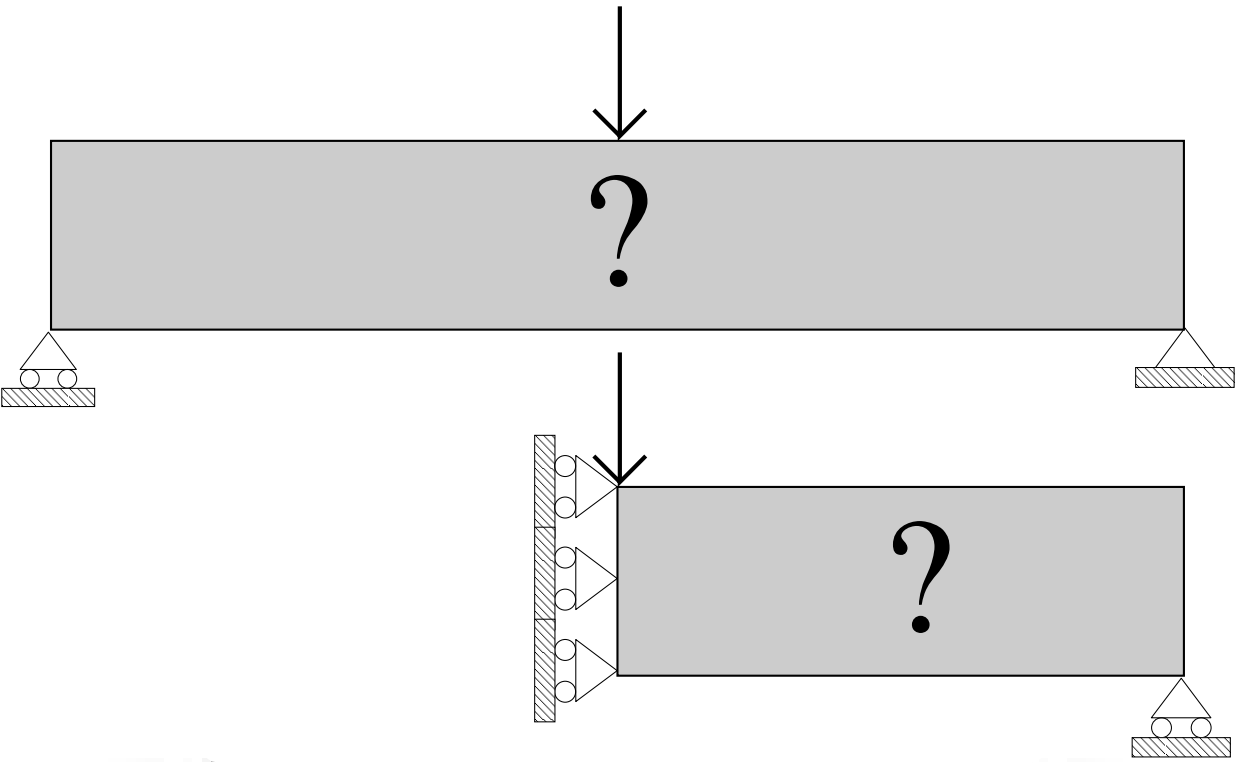
\includegraphics[width=0.6\textwidth]{./img/case_1.png}
    \caption{Initial structure for Case 1}
    \label{fig:case1_structure}
\end{figure}

In Figure \ref{fig:case1_1}, the results of the simulation for different values of $p$ and $r_{min}$ are shown.

\begin{figure}[H]
    \centering
    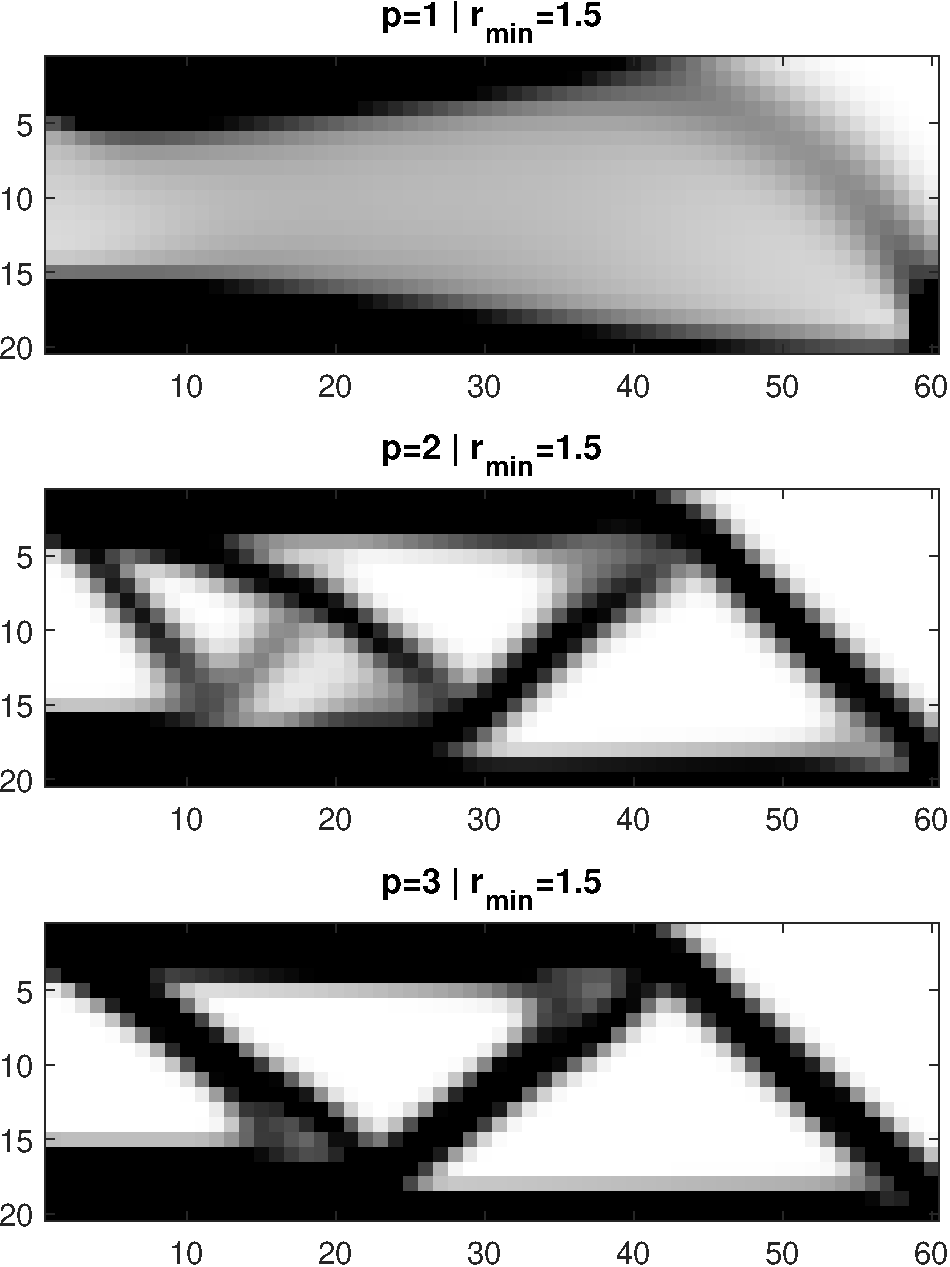
\includegraphics[width=0.49\textwidth]{./img/MATLAB/req_1p.pdf}
    \hfill
    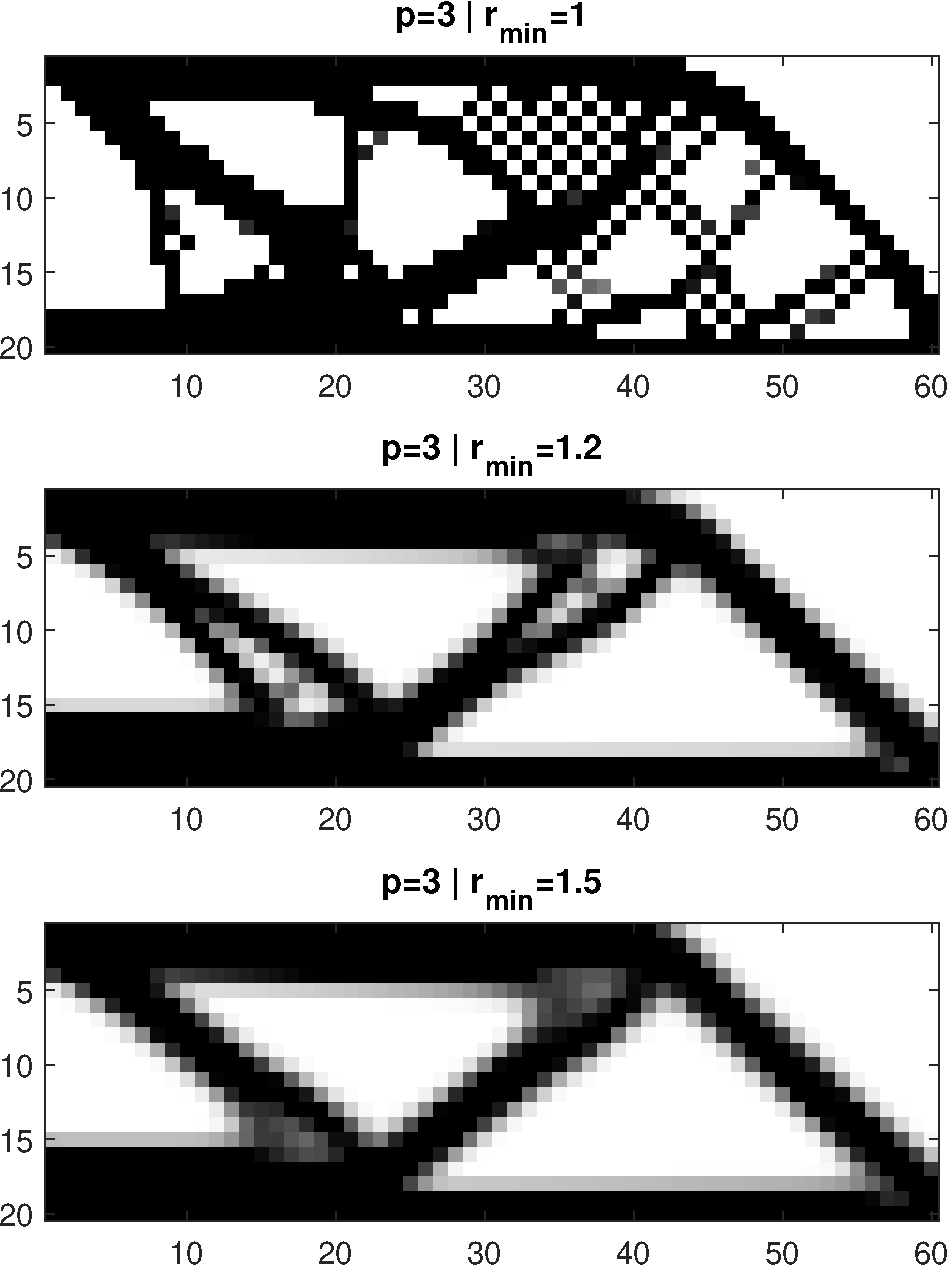
\includegraphics[width=0.49\textwidth]{./img/MATLAB/req_1rmin.pdf}
    \caption{Case 1: different $p$ and $r_{min}$ values.}
    \label{fig:case1_1}
\end{figure}

One can clearly see how the two parameters impact the final results.

The higher the $p$ value, the more pronounced the penalization of intermediate densities values.
By doing so, the algorithm is forced to find a solution with a more binary distribution of the material which is in general beneficial for a possible manufacturing process.

The $r_{min}$ parameter, which is the one controlling the filter radius, has also a significant impact on the final results.
For smaller values of $r_{min}$ the checkerboard pattern is clearly visible.



% Case 2
\subsection{Case 2: different boundary conditions}
\label{subsec:case2}

For this case, the considered structure is the one depicted in Figure \ref{fig:case2_structure}.

\begin{figure}[H]
    \centering
    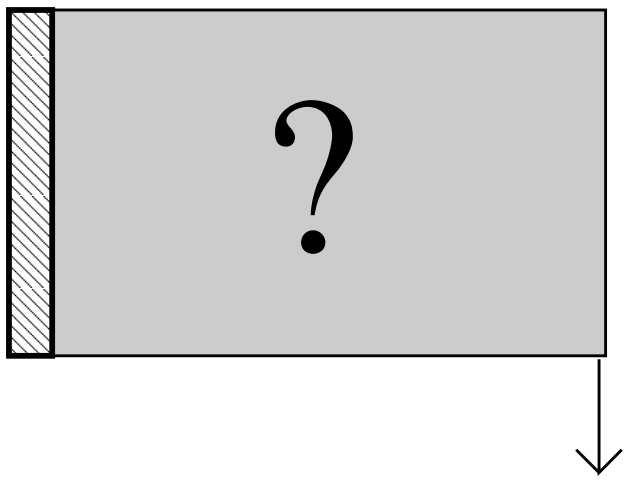
\includegraphics[width=0.3\textwidth]{./img/case_2.png}
    \caption{Initial structure for Case 2}
    \label{fig:case2_structure}
\end{figure}

In order to consider the different boundary conditions, the following lines of code were modified:

\begin{lstlisting}[style=Matlab-editor, firstnumber=79]
% DEFINE LOADS AND SUPPORTS (HALF MBB-BEAM)
F(2*(nelx+1)*(nely+1), 1) = -1;
fixeddofs = 1:2*(nely+1);
\end{lstlisting}

The optimized structure for the given loads and boundary conditions is shown in Figure \ref{fig:case2_1}.

\begin{figure}[H]
    \centering
    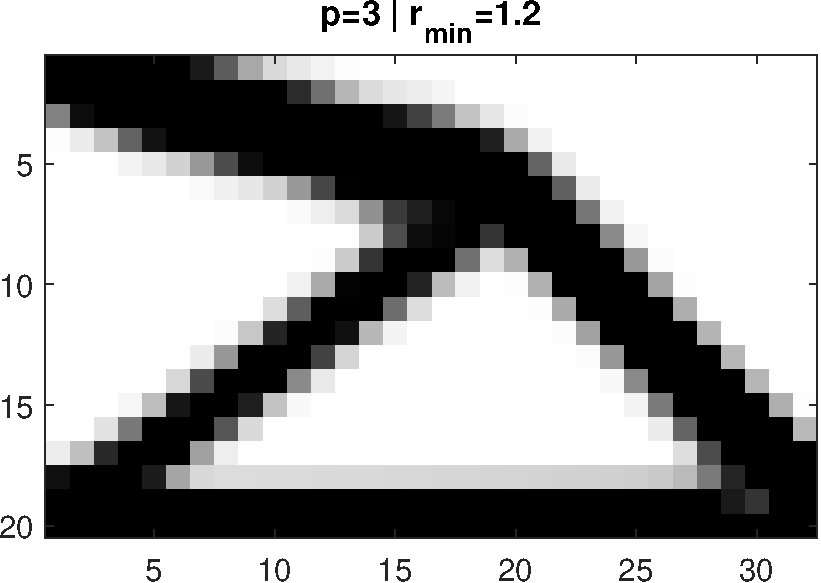
\includegraphics[width=0.5\textwidth]{./img/MATLAB/req_2.pdf}
    \caption{Case 2: different boundary conditions.}
    \label{fig:case2_1}
\end{figure}



% Case 3
\subsection{Case 3: multiple load cases}
\label{subsec:case3}

For this case, the considered structure is the one depicted in Figure \ref{fig:case3_structure}.

\begin{figure}[H]
    \centering
    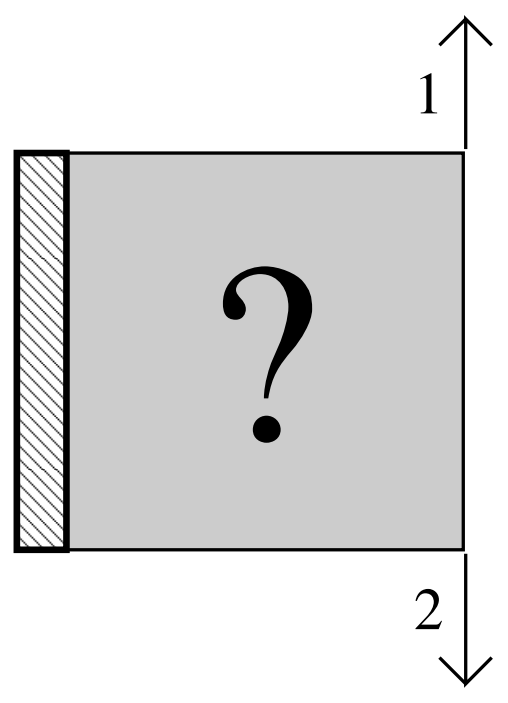
\includegraphics[width=0.25\textwidth]{./img/case_3.png}
    \caption{Initial structure for Case 3}
    \label{fig:case3_structure}
\end{figure}

Given the request, we now consider two different situations: one with the two loads applied simultaneously and one with the two loads applied separately.

When the loads are applied simultaneously, the following lines of code are used:

\begin{lstlisting}[style=Matlab-editor, firstnumber=79]
% DEFINE LOADS AND SUPPORTS (HALF MBB-BEAM)
F(2*(nelx+1)*(nely+1), 1) = -1;
F(2*(nelx)*(nely+1)+2, 1) = +1;
\end{lstlisting}

Instead, when the loads are applied separately, the following lines of code are used:

\begin{lstlisting}[style=Matlab-editor]
% Inside the Sensitivity Analysis computation
for i = 1:2
    Ue = U([ 2*n1-1; 2*n1; 2*n2-1; 2*n2; 2*n2+1; 2*n2+2; 2*n1+1; 2*n1+2 ], i);
    c = c + x(ely,elx)^p*Ue'*KE*Ue;
    dc(ely,elx) = dc(ely,elx) - p*x(ely,elx)^(p-1)*Ue'*KE*Ue;
end

% Inside the FE function
F = sparse(2*(nely+1)*(nelx+1), 2);
U = sparse(2*(nely+1)*(nelx+1), 2);

% DEFINE LOADS AND SUPPORTS (HALF MBB-BEAM)
F(2*(nelx+1)*(nely+1), 1) = -1;
F(2*(nelx)*(nely+1)+2, 2) = +1;
\end{lstlisting}

The optimized structures for the two situations are shown in Figure \ref{fig:case3_1}.

\begin{figure}[H]
    \centering
    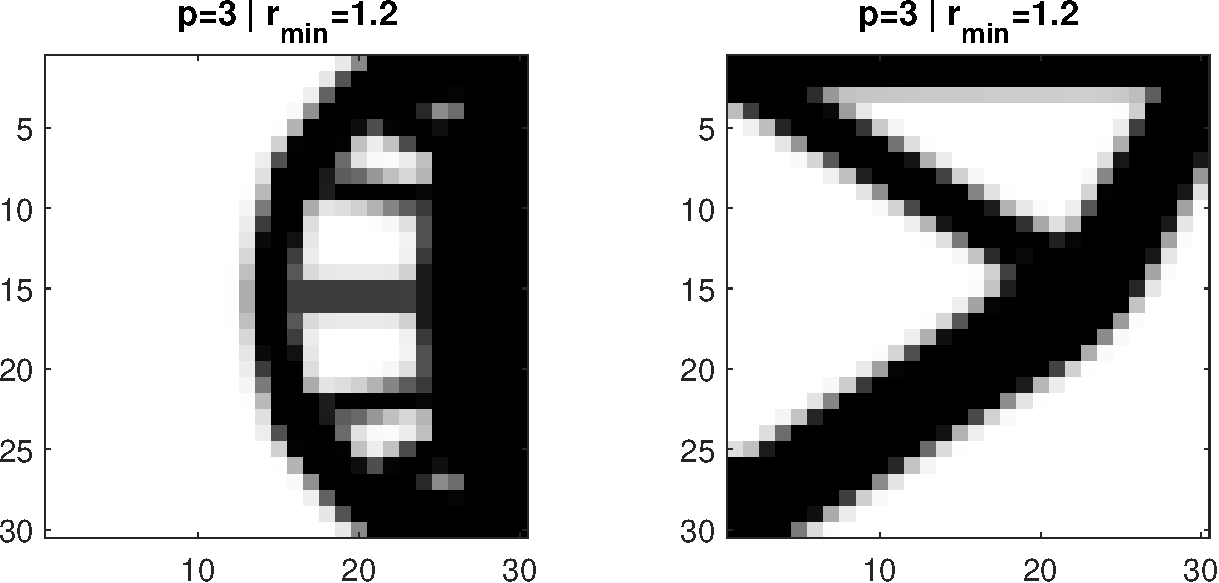
\includegraphics[width=0.8\textwidth]{./img/MATLAB/req_3.pdf}
    \caption{Case 3: simultaneous and separate loads cases.}
    \label{fig:case3_1}
\end{figure}

As we can see, the two different load situations lead to different optimized structures.

In particular, when the loads are applied simultaneously, the reaction forces are null and the structure is optimized as if there were no connection to the ground.
This also explains why the density of the structure is almost null in the left-hand side of the structure.

On the other hand, when the loads are applied separately, the reaction forces are not null and the structure is optimized accordingly.



% Case 4
\subsection{Case 4: passive elements}
\label{subsec:case4}

For this case, the considered structure is the one depicted in Figure \ref{fig:case4_structure}.

\begin{figure}[H]
    \centering
    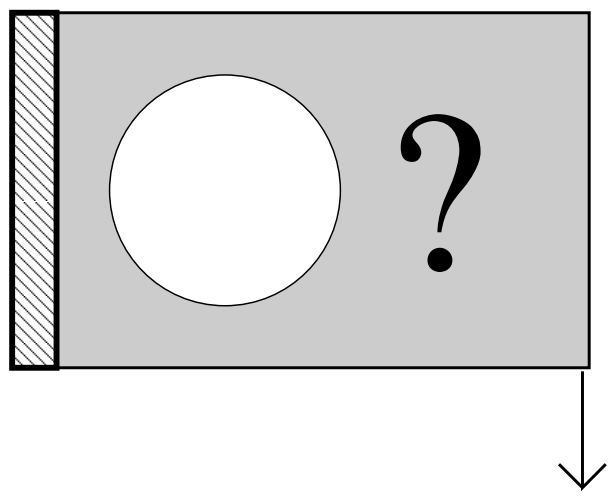
\includegraphics[width=0.3\textwidth]{./img/case_4.png}
    \caption{Initial structure for Case 4}
    \label{fig:case4_structure}
\end{figure}

To solve this problem we generate an array that defines which elements must be preserved.
This array should act as a map that restores the properties to be preserved for the required elements.

The following lines of code were added to the main script:

\begin{lstlisting}[style=Matlab-editor]
% Before the main optimization loop starts
passive = zeros(nely, nelx);
for ely = 1:nely
    for elx = 1:nelx
        if sqrt((ely-nely/2.)^2+(elx-nelx/3.)^2) < nely/3.
            passive(ely,elx) = 1;
            x(ely,elx) = 0.001;
        end
    end
end

% Inside the Optimality Criteria loop
xnew(passive == 1) = 0.001;
\end{lstlisting}

The optimized structure for this case is shown in Figure \ref{fig:case4_1}.

\begin{figure}[H]
    \centering
    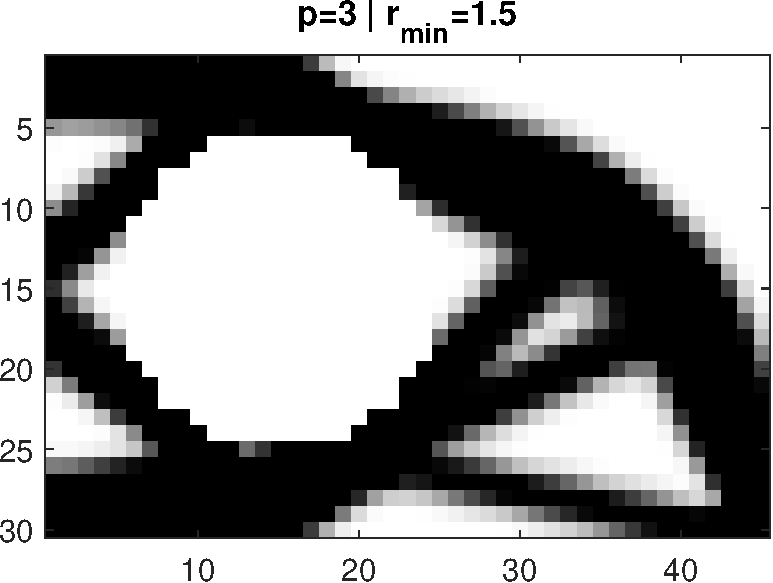
\includegraphics[width=0.5\textwidth]{./img/MATLAB/req_4.pdf}
    \caption{Case 4: passive elements.}
    \label{fig:case4_1}
\end{figure}